\documentclass{article}
\usepackage{hyperref}
\usepackage{times}
\usepackage[usenames,dvipsnames,svgnames,table]{xcolor}
\usepackage{color}
\usepackage{graphicx}
\graphicspath{ {./figures/} }
\usepackage[backend=bibtex, style=authoryear]{biblatex}
\addbibresource{C:/Users/ruesca/Documents/library/library.bib}
\usepackage{draftwatermark}
\interfootnotelinepenalty = 5000
\newcommand{\toolPar}[1]{\textcolor{red}{#1}}
\begin{document}
\title{Calculating a LiDAR-based "Erosion Score": An ArcGIS Toolbox Tutorial}
\author{Aaron Ruesch, Sarah Kempen, and Theresa Nelson\\
	Wisconsin Department of Natural Resources,\\
	101 S. Webster St.\\
	Madison, WI 53707-7921\\
	\href{Aaron.Ruesch@wisconsin.gov}{Aaron.Ruesch@wisconsin.gov}
}
\date{\today}
\maketitle
\begin{abstract}
	This document is a tutorial describing the steps required to calculate a spatially explicit erosion score based on a LiDAR digital elevation model (DEM). The erosion score is a bivariate index describing a landscape's relative vulnerability to sheet, rill, and gully erosion by incorporating information regarding topography, soils, rainfall, and land cover. The tools are intended for relatively small watersheds (less than 100 sq. km.) that have already been identified as watersheds that contribute higher non-point-source pollutant loads. For example, a hydrologic unit (HUC) that has been identified in a Total Maximum Daily Load (TMDL) model as a critical source area would be an appropriate place to use this tool. Presuming that the TMDL model has accurately identified the watershed as a pollutant source, we can further refine the prioritization to specific fields or sub-watersheds within the HUC12. With this framework, the intention is to prioritize the implementation of best-management practices on fields where pollutant loads are estimated to be the highest, thereby increasing the probability of improving downstream water quality using the fewest resources (i.e., "bang-for-buck" implementation).
\end{abstract}
\pagebreak
\tableofcontents
\listoftables
\listoffigures
\pagebreak
\section{Preparation}
	The tools were built for Wisconsin landscapes, and thus use data specific to Wisconsin, including post-processed LiDAR DEMs distributed by \href{http://relief.ersc.wisc.edu/wisconsinview/form.php}{WisconsinView}\footnote{http://relief.ersc.wisc.edu/wisconsinview/form.php}\label{wisconsinViewWebsite} and Wisconsin-specific coordinate systems (Wisconsin Transverse Mercator). In terms of software, the tools require ArcGIS 10.0 or later, the Spatial Analyst extension, and an optimized DEM fill tool that can be downloaded \href{http://tools.crwr.utexas.edu/OptimizedPitRemoval/Optimized-Pit-Removal-V1.5.1.zip}{here}\footnote{http://tools.crwr.utexas.edu/OptimizedPitRemoval/Optimized-Pit-Removal-V1.5.1.zip}. In terms of data, you will need LiDAR data downloaded from \href{http://relief.ersc.wisc.edu/wisconsinview/form.php}{WisconsinView}\footnotemark[1], a feature class polygon for the boundary of your area of interest (recommended smaller than 100 sq. km.), \href{http://www.mrlc.gov/nlcd06_data.php}{NLCD land-cover data}\footnote{http://www.mrlc.gov/nlcd06\_data.php}\label{nlcdWebsite}, \href{http://datagateway.nrcs.usda.gov/GDGOrder.aspx?order=QuickState}{gSSURGO soils data}\footnote{http://datagateway.nrcs.usda.gov/GDGOrder.aspx?order=QuickState}\label{nrcsWebsite}, and optionally, the \href{http://www.fsa.usda.gov/FSA/apfoapp?area=home&subject=prod&topic=clu}{USDA common land unit dataset (CLU)}\footnote{http://www.fsa.usda.gov/FSA/apfoapp?area=home\&subject=prod\&topic=clu}. To download the CLU dataset, you must be a FSA/NRCS/RD\footnote{Farm Service Agency, Natural Resources Conservation Service, Rural Development} employee. If you are not employed by one of these agencies, you may use an alternate boundary for summarization (e.g., parcels, sub-watersheds). Running the tools will likely require a moderate-to-high level of familiarity with GIS concepts and ArcGIS Desktop software.
	\begin{enumerate}
		\item \emph{Load the tools into ArcGIS}: Open ArcMap. Navigate to ArcToolbox. Right-click on \toolPar{ArcToolbox} then click \toolPar{Add Toolbox}. Navigate to the \toolPar{-- LiDAR Erosion Score --.tbx} file stored in the root directory of the distributed toolbox.
		\item \emph{Define an area of interest}: The area of interest, for the purpose of water quality improvement, will likely be a watershed boundary, and therefore will be referred to as the "watershed" within this document. Watershed boundaries are available on the internet through USGS---the finest-scale watershed boundaries that are available are \href{http://water.usgs.gov/GIS/huc.html}{Hydrologic Unit Codes level 12 (HUC12s)}\footnote{http://water.usgs.gov/GIS/huc.html}. The DNR has an internal version of HUC16 delineations that is available upon request. If no watershed boundary exists, you can manually digitize a boundary using the LiDAR DEM or contours if they are availabe.
		\item \emph{Download the gSSURGO soils database}: Go to the NRCS \href{http://datagateway.nrcs.usda.gov/GDGOrder.aspx?order=QuickState}{GeoSpatialDataGateway} 'Order by State' website. Under \toolPar{Select State}, choose \toolPar{Wisconsin}. You will be prompted to select a dataset---scroll down to \toolPar{Soils} and choose \toolPar{Gridded Soil Survey Geographic (gSSURGO) by State} and click \toolPar{CONTINUE}, then \toolPar{CONTINUE} again. Fill in the form with your personal information and click \toolPar{CONTINUE} and \toolPar{PLACE ORDER}. An email will be sent to you when your order is ready. Find the FTP site in the email, download the associated zip file, and unzip it. There will be another zip file in the resulting directory---unzip that as well and note the location of \toolPar{[zip directory]/soils/Wisconsin/SDM\_State\_WI.gdb}.
		\item \emph{Download the NLCD2006 land-cover raster}: Go to the \href{http://www.mrlc.gov/nlcd06_data.php}{Multi-Resolution Land Characteristics Consortium (MRLC)} download website for NLCD2006 and click the top link under \toolPar{Conterminous United States} labeled \toolPar{NLCD2006 Land Cover}. The data should immediately begin downloading. When the download is complete, unzip the file and note the location of \toolPar{nlcd2006\_landcover\_4-20-11\_se5.img}.
		\item \emph{Download LiDAR DEM(s)}: Go to the \href{http://relief.ersc.wisc.edu/wisconsinview/form.php}{WisconsinView Data Portal} (see link on page~\pageref{wisconsinViewWebsite}. If this is your first time visiting the WisconsinView Data Portal, fill in the form at the bottom of the page with your personal information, click \toolPar{LiDAR DEMs}, accept the disclaimer, and click \toolPar{Submit}. Click the county(s) where your watershed is located. This will direct you to an FTP site---click the zip file in the top level directory. Unzip the file and note the location where the resulting directory was stored.
	\end{enumerate}
\section{Tools}
	\subsection{Condition the DEM}
		To properly describe how water moves across your watershed, we must first "condition" the DEM (methods based on \cite{vaughn_method_2010}), which means to remove presumed errors in elevation so that the GIS model of hydrology can correctly infer the direction of flow based on changes in elevation.
		
		One of the major barriers in this process is correctly modeling the flow of water through culverts and bridges. Therefore, we have to first manually digitize all culverts and bridges in our watershed where flowpaths are not properly reprsented by the DEM. The majority of these cases will occur where road berms were built. These topographies create "digital dams" that prevent the hydrologic model from appropriately describing downslope flow. 
		
		To eliminate digital dams, we will digitize each culvert as a polyline feature following these steps (see Figure ~\ref{fig:digitizingCulverts}):
		\begin{enumerate}
			\item Create a "filled" DEM using the \toolPar{Fill} tool in ArcGIS Spatial Analyst and subtract the original DEM from the filled DEM to create a raster of the depression depths. Alternatively, you can type this snippet of code into the ArcGIS Desktop Python window (
\includegraphics[scale=0.8,natwidth=16,natheight=13]{pythonIcon.png}):\\\\
			\texttt{from arcpy.sa import *}\\
			\texttt{dem = "C:/path/to/dem"}\\
			\texttt{depressionDepth = "C:/path/to/depressionDepth"}\\
			\texttt{depressionDepth = Fill(dem) - Raster(dem)}\\
			\texttt{depressionDepth.save(depressionDepth)}\\\\
			replacing \texttt{"C:/path/to/dem"} and \texttt{"C:/path/to/depressionDepth"} with the file paths for your LiDAR DEM and the output raster for inferring where depressions lie.
			\item Deep depressions near road berms are places where a culvert is probably located. Locate one of these depressions using the depression-depth raster from above, then zoom to it.
			\item To visualize digital dams, open the \toolPar{Symbology} tab in the \toolPar{Layer properties} window for the original DEM. Choose the \toolPar{Stretched} option using \toolPar{From Current Display Extent} within the \toolPar{Statistics} box, and choose a color gradient that spans multiple hues (e.g., a rainbow color scheme).
			\item Create an empty polyline feature class.
			\item Start an editing session on the empty polyline feature class.
			\item Each polyline feature should only have two nodes. The nodes need to be drawn in order, from upstream to downstream, across the digital dam. 
			\item Use the rainbow-colored DEM to locate the lowest elevation DEM gridcell on the upstream side of the digital dam. Digitize the upstream node on the center of that cell.
			\item Next, locate a DEM gridcell on the downstream side of the digital dam that has lower elevation than the gridcell underlying the upstream node. Digitize the downstream node on the center of that cell and finish the feature.
			\item Repeat until all digital dams have culvert features spanning across them.
		\end{enumerate}
		A correctly digitized polyline will inform a DEM interpolation routine that the digital dam should be "cut" along the geometry of the culvert feature according to the slope of the elevation between the DEM gridcells on the up- and downstream side of the digital dam.
		
		After all culverts have been digitized, open the \toolPar{Condition the LiDAR DEM} tool in the \toolPar{LiDAR Erosion Score} toolbox. Add the \toolPar{Culverts} polyline feature class, the \toolPar{Watershed area} polygon feature class, and the \toolPar{Raw LiDAR DEM} raster dataset that you downloaded from \href{http://www.wisconsinview.org/}{WisconsinView}. The tool also asks for the \toolPar{Optimized fill software executable}; after decompressing the downloaded \href{http://tools.crwr.utexas.edu/OptimizedPitRemoval/Optimized-Pit-Removal-V1.5.1.zip}{optimized fill software}\footnote{http://tools.crwr.utexas.edu/OptimizedPitRemoval/Optimized-Pit-Removal-V1.5.1.zip}, choose the \toolPar{OptimizedPitRemoval.exe} file from the resulting directory. Finally, define an \toolPar{Output conditioned DEM} and an \toolPar{Output optimized fill}. The \toolPar{Output conditioned DEM} will be a raster file that has minor errors and digital dams removed. It will have a coarsened cellsize of 3 meters (unless the cell size was manually changed in the \toolPar{Environment settings}). The \toolPar{Output optimized fill} will be a DEM that has all "pits" (depressions) removed where water would theoretically pool. That is, the resulting elevation model has no seepages or wetlands that store water---all water runs off.
	\subsection{Identify Internally Draining Areas}
		Because the eroded soil that flows into internally draining areas (also known as "non-contributing areas") does not contribute to water quality problems in terms of suspended solids, these areas will eventually be removed from the erosion score (ES) model. But first, the extent of internally draining areas must be identified.
		
		We assume that internally draining areas are areas where the volume of the depression on the landscape is large enough to store the runoff produced from a precipitation event as large as a specified storm event. To model runoff, we use a "curve number" approach in which the proportion of precipitation that results in runoff is based on land cover and hydrologic soil group.
		\subsubsection{Prepare Precipitation Data}
			To identify internally draining areas, we need raster precipitation data describing a depth of rain that will be used to define the volume threshold (i.e., capacity) of each internally draining area. The depth of rain is specified in the tool by the frequency of occurence (in units of years) of a specified duration of storm (in units of hours). For example, a frequency of value 10 and duration of value 24 represents the 10-year 24-hour rainfall event. The tool will automatically download raster data from NOAA's \href{http://dipper.nws.noaa.gov/hdsc/pfds/}{Precipitation Frequency Data Server}\footnote{http://dipper.nws.noaa.gov/hdsc/pfds/}. The resulting precipitation raster will be in thousandths of inches
		
			In ArcToolbox, expand the \toolPar{LiDAR Erosion Score} toolbox and double-click the \toolPar{Download Precipitation Data} script tool. Define the \toolPar{Frequency} and \toolPar{Duration} of storm. Then choose a \toolPar{Raster template} (usually the DEM for the watershed) which will define the cell size, grid, extent, and mask of the resulting precipitation depth raster. Finally, define an \toolPar{Output precipitation raster}.
		\subsubsection{Create a curve number raster}
			Open the \toolPar{Create Curve Number Raster} tool. For \toolPar{Curve number table}, find the database file (extension .dbf) called \toolPar{curveNumberTable.dbf}---it will be in the root directory of the folder where the distributed tools are located. This table includes curve numbers for each unique combination of NLCD class and SSURGO hydrologic soil group (see Table ~\ref{table:curveNumberTable} taken from \cite{mcenroe_storm_2003}). For the \toolPar{NLCD raster}, browse for the version of NLCD2006 that you downloaded. For the \toolPar{gSSURGO geodatabase}, point to the \toolPar{SDM\_State\_WI.gdb} file geodatabase that you downloaded from the NRCS GeoSpatialDataGateway (see Preperation). Finally, add the \toolPar{Conditioned DEM} from tool 1 (to use as a grid template) and define an output \toolPar{Curve number raster}.
			
			We will use the NLCD land cover data to create a raster surface of curve numbers. First, clip your version of NLCD to the extent of the \toolPar{Output conditioned DEM} from tool 1, \toolPar{Condition the LiDAR DEM}. Then, add a field to the clipped NLCD raster to store a curve number value associated with each land cover class. There is some debate over what curve numbers should be used for each land cover type (and generally whether curve numbers can effectively be applied to satellite-based land-cover classes).
		\subsubsection{Run the tool}
			After you have created a curve number raster, you are ready to run the tool for identifying internally draining areas. Open the \toolPar{Identify Internally draining Areas} tool in the \toolPar{LiDAR Erosion Score} toolbox. Add the \toolPar{Conditioned DEM} and \toolPar{Optimized fill raster} from tool 1, the \toolPar{Precipitation frequency-duration raster} from tool 2a, the \toolPar{Curve number raster} you just created, and the \toolPar{Watershed area} polygon. Finally, define an \toolPar{Output internally draining areas} raster (a raster with unique, but arbitrary, IDs for each internally draining watershed) and an \toolPar{Output DEM excluding internally draining areas}. The \toolPar{Output DEM excluding internally draining areas} is simply the conditioned DEM with the extent of internally draining areas set to \emph{NoData}.
	\subsection{Recondition DEM for Internally draining Areas}
		Creating a hydrologically valid DEM is dependent on the extent of DEM cells. Often, the DEM cells are coerced to model "outward" flow on the edge of the DEM raster, presuming that the edge of the raster defines an area outside of the watershed. To properly model internally draining areas, we have to recondition the DEM to force the direction of hydrologic flow \emph{toward} the internally draining area. Thus, accumulating flow will not be propogated downstream of the internally draining area. That is, flow that enters a internally draining area will "dissappear."
		
		To hydrologically correct for internally draining areas, open the \toolPar{Recondition DEM for Internally draining Areas} tool. Add the \toolPar{DEM excluding internally draining areas} from tool 2c. You may also optionally add \toolPar{Additional internally draining areas}, which could include any features on the landscape that could eliminate runoff, such as grass waterways, strip cropping, or any other best-management practices (BMPs) that would eliminate runoff that can be identified spatially. These features should be rasterized to the cellsize, extent, and grid (i.e., "snapped") of the \toolPar{DEM excluding internally draining areas}. Next, find the path to the \toolPar{Optimized fill software executable} as you did in tool 1. Finally, define an \toolPar{Output Reconditioned DEM excluding internally draining areas}. This DEM will be the final DEM used to estimate the ES.
	\subsection{Calculate Stream Power Index}
		The first metric in the bivariate ES is the "stream power index." The stream power index includes information on slope and upstream drainage area---it is used for estimating the locations of gully erosion:
		\begin{equation}
			SI_{i} = ln(DA_{i} \times tan(G_{i}))
		\end{equation}
		where $SI$ is the stream power index at gridcell $i$, $DA$ is the upstream drainage area (flow accumulation at gridcell $i$ multiplied by gridcell area), and $G$ is the slope at a gridcell $i$ in radians.
		
		Open the \toolPar{Calculate Stream Power Index} tool in the \toolPar{LiDAR Erosion Score} toolbox. Add the \toolPar{Conditioned DEM} from tool 1. This input will be used to calculate slope, so you do not want to confuse this input with any "filled" DEM---filled DEM are used only for modeling hydrologic flow, and thus should not be used to calculate other topographic metrics such as slope. Add the \toolPar{Reconditioned DEM excluding internally draining areas} from tool 3. This input will be used to calculate drainage area using a "flow accumulation" raster. Assign a \toolPar{Flow accumulation threshold}---this value sets the number of upstream gridcells for which the flow is assumed to transition to surface water\footnote{This value will vary depending on the cell size of your DEM and the type of hydrology in your area of interest. The default 50,000 was chosen by surveying a watershed in Southern Wisconsin and determining the number of pixels on a 3-meter resolution flow accumulation raster where hydrology transitioned to surface water. The same approach was used on a watershed in Northern Wisconsin using a 10-meter resolution flow accumulation raster and the flow accumulation threshold was determined to be 5,000. Assuming a linear relationship between cell size and flow accumulation threshold, we can derive a relationship using these two cases as a guide for setting the threshold: $FAC = -6.5CS + 70$ where $FAC$ is the flow accumulation threshold in thousands of pixels and $CS$ is the cell size of the DEM in meters.}. The stream power index is intended to only model landscape erosion, not instream or bank erosion, and thus gridcells assumed to be surface water should be excluded. Finally, define an \toolPar{Output stream power index raster}.
	\subsection{Calculate Soil Loss Using the Universal Soil Loss Equation (USLE)}
		\subsubsection{Overview of the USLE}
			The second metric in the bivariate ES is soil loss as estimated by the USLE. The USLE estimates sheet and rill erosion across fields using:
			\begin{equation}
				E_{i} = R_{i} \times K_{i} \times LS_{i} \times C_{i} \times P_{i}
			\end{equation}
			where at each gridcell $i$, $E$ is soil loss in $tons \cdot (ha \cdot year)^{-1}$, $R$ is rainfall erosivity in $(megajoule \cdot millimeter) \cdot (ha \cdot hour \cdot year)^{-1}$, K is soil erodibility in $(tons \cdot ha \cdot hour) \cdot (ha \cdot megajoule \cdot mm)^{-1}$, $LS$ is slope/slope-length (dimensionless), $C$ is a land cover factor (unitless), and $P$ is a "practice" factor (unitless metric describing the capacity of a land-management practice to prevent erosion) which is beyond the scope of this tool and thus will assumed to be 1. All these data need to be acquired prior to running the tool, and will take some time to prepare. Preparation steps are outlined below in detail.
		\subsubsection{Prepare GIS datasets}
			Rainfall erosivity (or R-factor) is the cumulative force of rainfall on soil. In Wisconsin where topographic effects to rainfall intensity are minimal, erosivity varies at very large spatial scales. Because this tool is intended for small watersheds, erosivity can safely be assumed to be constant. For an appropriate constant value of erosivity, see \cite{u.s._e.p.a._stormwater_2005} Fact Sheet 3.1 page 5 for a map of erosivity in U.S. customary units. Multiply this value by 17.02 to convert to international (SI, or metric) units. Alternatively, if you know \emph{a priori} that erosivity varies at a scale within the extent of your watershed, you can define an \toolPar{Erosivity raster}. If you choose to use an \toolPar{Erosivity raster}, resample the grid to the extent and resolution of the \toolPar{Conditioned DEM} from tool 1---ensure that the resampled grid matches the grid of the \toolPar{Conditioned DEM} by setting the \toolPar{Snap Raster} to the \toolPar{Conditioned DEM} in the \toolPar{Environment settings} of the \toolPar{Resample} tool.
			
			Erodibility, or "K-factor," is an attribute that can be found in the gSSURGO soils database. Open the \toolPar{Rasterize K-factor for USLE} tool in the \toolPar{LiDAR Erosion Score} toolbox. Under \toolPar{gSSURGO geodatabase}, point to the \toolPar{SDM\_State\_WI.gdb} file geodatabase that you downloaded from the NRCS GeoSpatialDataGateway (see Preperation). Keep the \toolPar{K-factor} field as the default \toolPar{kwfact}. Add the \toolPar{Conditioned DEM} to use as a template for the resulting K-factor raster and the \toolPar{Watershed area} polygon used to clip the DEM (these are the same two inputs from tool 1). Finally, define an \toolPar{Output K-factor raster} and run the tool.
			
			The last step in preparing the GIS datasets for calculating soil loss is creating a \toolPar{C-factor raster}. The C-factor is a unitless metric that adjusts the amount of soil loss for different land cover types. To create the C-factor raster, we will simply reclassify the NLCD2006 land cover codes to a meaningful C-factor value. Example C-factors are listed in Table ~\ref{table:cFactorTable} (taken from \cite{montana_deq_draft_2012}, Appendix F). Open the \toolPar{Reclassify} tool in the \toolPar{ArcToolbox}. Define the \toolPar{Input raster} as the NLCD2006 and the \toolPar{Reclass field} as \toolPar{Value}. Manually input the old-to-new reclassification in the provided \toolPar{Reclassification} interface. The new values can only be integers, so enter the desired C-factors after multiplying by 1000. Define an \toolPar{Output raster} and run the tool. The resulting C-factor raster will need to be reconverted to a decimal number. Open the \toolPar{Raster Calculator} tool in \toolPar{Spatial Analyst Tools/Map Algebra}. In the \toolPar{Map Algebra expression} box, enter the following command:\\\\\texttt{Float("C:\textbackslash{}cFactorTimes1000") / 1000}\\\\where \texttt{"C:\textbackslash{}cFactorTimes1000"} is the path to the reclassified raster from above. The resulting \toolPar{Output raster} will be used as an input to the \toolPar{Calculate Soil Loss Using USLE} tool.
		\subsubsection{Run the tool}
			Open the \toolPar{Calculate Soil Loss Using USLE} tool in the \toolPar{LiDAR Erosion Score} toolbox. Add the \toolPar{Conditioned DEM} from tool 1, and the \toolPar{Reconditioned DEM excluding internally draining areas} from tool 3. If you decide to use a raster version of erosivity, add that dataset to the \toolPar{Erosivity raster} parameter. On the contrary, if erosivity can be considered constant, add that value to the \toolPar{Erosivity constant} box. In either case, use an erosivity value in SI units of $(megajoule \cdot millimeter) \cdot (ha \cdot hour \cdot year)^{-1}$. You will notice that both erosivity parameters are considered optional---if no value is given, an erosivity value of 1 will be used. If an erosivity value of 1 is used, the ES will be the same as if you had entered a \toolPar{Erosivity constant}, however the resulting soil loss raster cannot be interpreted on an absolute scale. Next, add both the \toolPar{K factor raster} calculated from gSSURGO and the \toolPar{C Factor raster} calculated from NLCD. The \toolPar{C factor raster} is considered optional---if no value is given, the C factor is given a value of 1. As you did in tool 4, define a \toolPar{Flow accumulation threshold}\footnotemark[10] to set the number of upstream gridcells for which the flow is assumed to transition to surface water. Finally, define an output soil loss raster. If all inputs were in SI units, and all optional inputs were set to a meaningful value, the output will be in units of $tons \cdot (ha \cdot year)^{-1}$.
	\subsection{Calculate Erosion Score}
		The ES is a bivariate index based on the stream power index and USLE-based soil loss. The ES gives equal weight to both by first, normalizing the distribution of soil loss by log-transforming (the stream power index is already normalized), second, centering their distribution on 0 and forcing the standard deviation to 1 by calculating a Z-score\footnote{$Z = (x_{i} - \mu) / \sigma$ where $x$ is the pixel value of the $i^{th}$ pixel, $\mu$ is the mean of the raster dataset, and $\sigma$ is the standard deviation of the raster dataset}, and finally taking the average of the Z-scores of the soil loss and the stream power index. Therefore, ES can be interpreted as the number of standard deviations from the mean. As a standard benchmark, an ES above 2 is above the 95th percentile of all pixels.
		
		Open the \toolPar{Calculate Erosion Score} tool. Add the \toolPar{Soil loss raster} from tool 5b and the \toolPar{Stream power index raster} from tool 4. You may optionally add a \toolPar{Zonal statistic boundary feature class} if you choose to summarize the ES---the natural boundary in this case would be the CLU field boundaries. If you choose to summarize by a zones, you must choose a \toolPar{Zonal statistic field} (if the \toolPar{Zonal statistic field} is a string/text data type, the zone values will be coerced to sequential integers). Next, add the \toolPar{Output erosion score raster} and \toolPar{Output summary table} optional outputs. The \toolPar{Output summary table} is required if a \toolPar{Zonal statistic boundary feature class} was defined. Finally, select whether you would like to \toolPar{Aggregate polygons}; if you choose to aggregate polygons, the \toolPar{Zonal statistic boundary feature class} will dissolve zones that are less than the median area into neighboring polygons. This feature allows us to better interpret \emph{total} erosion without biasing larger area zones.
\section{Interpretation and Limitations}
	Congratulations! If you have read this far, it hopefully means that you have an ES raster layer and likely an ES summarized by agricultural field. These results can help you prioritize where to focus your efforts for improving water quality in your watershed \underline{and} downstream. 
	
	If you defined an \toolPar{Output summary table} in the \toolPar{Calculate Erosion Score} tool, you will have a table of summary statistics of erosion scores that you can join to your \toolPar{Zonal statistic boundary feature class} to locate priority features by creating color maps of different statistics using quantitative symbology on your boundary feature class. The summary table will have several statistics to choose from including the mean, maximum, and sum of all erosion score values within the boundaries of each feature. If you are most concerned with highly concentrated erosion, perhaps the most valuable statistic would be the mean erosion score, however the mean erosion score may reflect anomolous high values that skew the average---this is particularly a problem in small fields. If you are most concerned with total sediment runoff, perhaps the best statistic would be the sum, however the sum erosion score may reflect simply the size of the field, which may obscure otherwise priority fields that are smaller, but have more intense runoff events. If you are interested in the highest intensity runoff areas, you may be interested in the maximum erosion score, however this statistic may have the same problem with interpretation as the mean statistic---it may reflect anomolous high pixels, particularly in small fields. There are several ways to look at the resulting data, and no single statistic gives the correct answer. We advise the user to explore each of these statistics for different insights regarding erosion processes in your area of interest.
	
	This dataset is best interpreted in combination with other determining factors of erosion and/or nutrient runoff. For example, as a watershed manager, you may be interested in what cropping practices are present---if information regarding specific practices are availabe and a P-factor can be inferred, these practices can be used to modify the USLE by multiplying a P-factor raster by the USLE raster. Additionally, you may be interested in fields that are on or near surface water---the ES summarized by field can be overlaid on a feature layer with information regarding the location of perennial or intermittent streams to gain insight into the potential for sediment delivery and transport.
	
	Although the ES data product can be useful for prioritizing areas for implementation of BMPs, there are several key limitations that decision-makers should be aware of when interpreting the data. First, the ES is a unitless index. Although the output of the USLE raster is intended to have value in terms of total soil loss in $tons \cdot (ha \cdot year)^{-1}$, the stream power index raster does not. Because the two are combined into a single index, the resulting raster cannot be interpreted absolutely; differences from field-to-field can only be interpreted ordinally. Therefore, this tool cannot be used to make inferences regarding the water quality improvement associated with the implementation of BMPs, but only to make decisions about where to prioritize implementation. Second, the ES itself has not been rigorously validated. Calculating erosion using a GIS is a relatively new science---there are many case studies investigating soil loss using a GIS-based USLE and a few studies identifying gullies using the stream power index. The results of these studies are mixed in terms of prediction accuracy, and there are no meta-analyses to date that broadly investigate the utility of either metric. Finally, the ES is only intended to facilitate prioritization of the implementation of BMPs in regions where erosion is the dominant source of water quality impairments. If water quality impairments are due to some other source, such as the mis-application of liquid manure, the usage of the ES for prioritization may lead managers to implement BMPs on low-priority fields. Because of the above limitations, this tool cannot be used to predict erosion \emph{rates}, but rather the relative probability of a field to have \emph{more} erosion problems than its neighbors.
\pagebreak
\printbibliography
\pagebreak
\section*{Tables}
	\begin{table}[h]
		\centering
		\begin{tabular}{clc}
			\hline
			NLCD Code & Description & C-Factor\\
			\cline{2-3}
			11 & Open Water & 0 \\
			21 & Developed, Open Space & 0.003 \\
			22 & Developed, Low Intensity & 0.001 \\
			23 & Developed, Medium Intensity & 0.001 \\
			24 & Developed, High Intensity & 0.001 \\
			31 & Barren Land (Rock/Sand/Clay) & 0.001 \\
			41 & Deciduous Forest & 0.003 \\
			42 & Evergreen Forest & 0.003 \\
			43 & Mixed Forest & 0.003 \\
			52 & Shrub / Scrub & 0.02 \\
			71 & Grassland / Herbaceous & 0.02 \\
			81 & Pasture / Hay & 0.02 \\
			82 & Cultivated Crops & 0.2 \\
			90 & Woody Wetlands & 0.013 \\
			95 & Emergent Herbaceous Wetlands & 0.003 \\
			\hline
		\end{tabular}
		\caption[Cover factors (C-factors) for the Universal Soil Loss Equation (USLE)]{Cover factors (C-factors) for the Universal Soil Loss Equation (USLE) based on land-cover classifications of the National Land Cover Dataset (NLCD) (\cite{montana_deq_draft_2012})}
		\label{table:cFactorTable}
	\end{table}
	\begin{table}[h]
		\centering
		\begin{tabular}{lcccc}
			\multicolumn{1}{c}{ } & \multicolumn{4}{c}{Hydrologic Soil Group} \\
			NLCD Code and Description & A & B & C & D \\
			\hline
			11 Open Water & 100 & 100 & 100 & 100 \\
			21 Developed, Open Space & 89 & 92 & 94 & 95 \\
			22 Developed, Low Intensity & 57 & 72 & 81 & 86 \\
			23 Developed, Medium Intensity & 61 & 75 & 83 & 87 \\
			24 Developed, High Intensity & 89 & 92 & 94 & 95 \\
			31 Barren Land (Rock/Sand/Clay) & 77 & 86 & 91 & 94 \\
			41 Deciduous Forest & 36 & 60 & 73 & 79 \\
			42 Evergreen Forest & 36 & 60 & 73 & 79 \\
			43 Mixed Forest & 36 & 60 & 73 & 79 \\
			52 Shrub / Scrub & 35 & 56 & 70 & 77 \\
			71 Grassland / Herbaceous & 49 & 69 & 79 & 84 \\
			81 Pasture / Hay & 49 & 69 & 79 & 84 \\
			82 Cultivated Crops & 67 & 78 & 85 & 89 \\
			90 Woody Wetlands & 36 & 60 & 73 & 79 \\
			95 Emergent Herbaceous Wetlands & 49 & 69 & 79 & 84 \\
			\hline
		\end{tabular}
		\caption[Curve numbers for estimating runoff]{Curve numbers for estimating runoff based on National Land Cover Dataset (NLCD) classifications and Soil Survey Geographic Database (SSURGO) hydrologic soil groups (\cite{mcenroe_storm_2003})}
		\label{table:curveNumberTable}
	\end{table}
\clearpage
\section*{Figures}
	\begin{figure}[h]
		\centering
		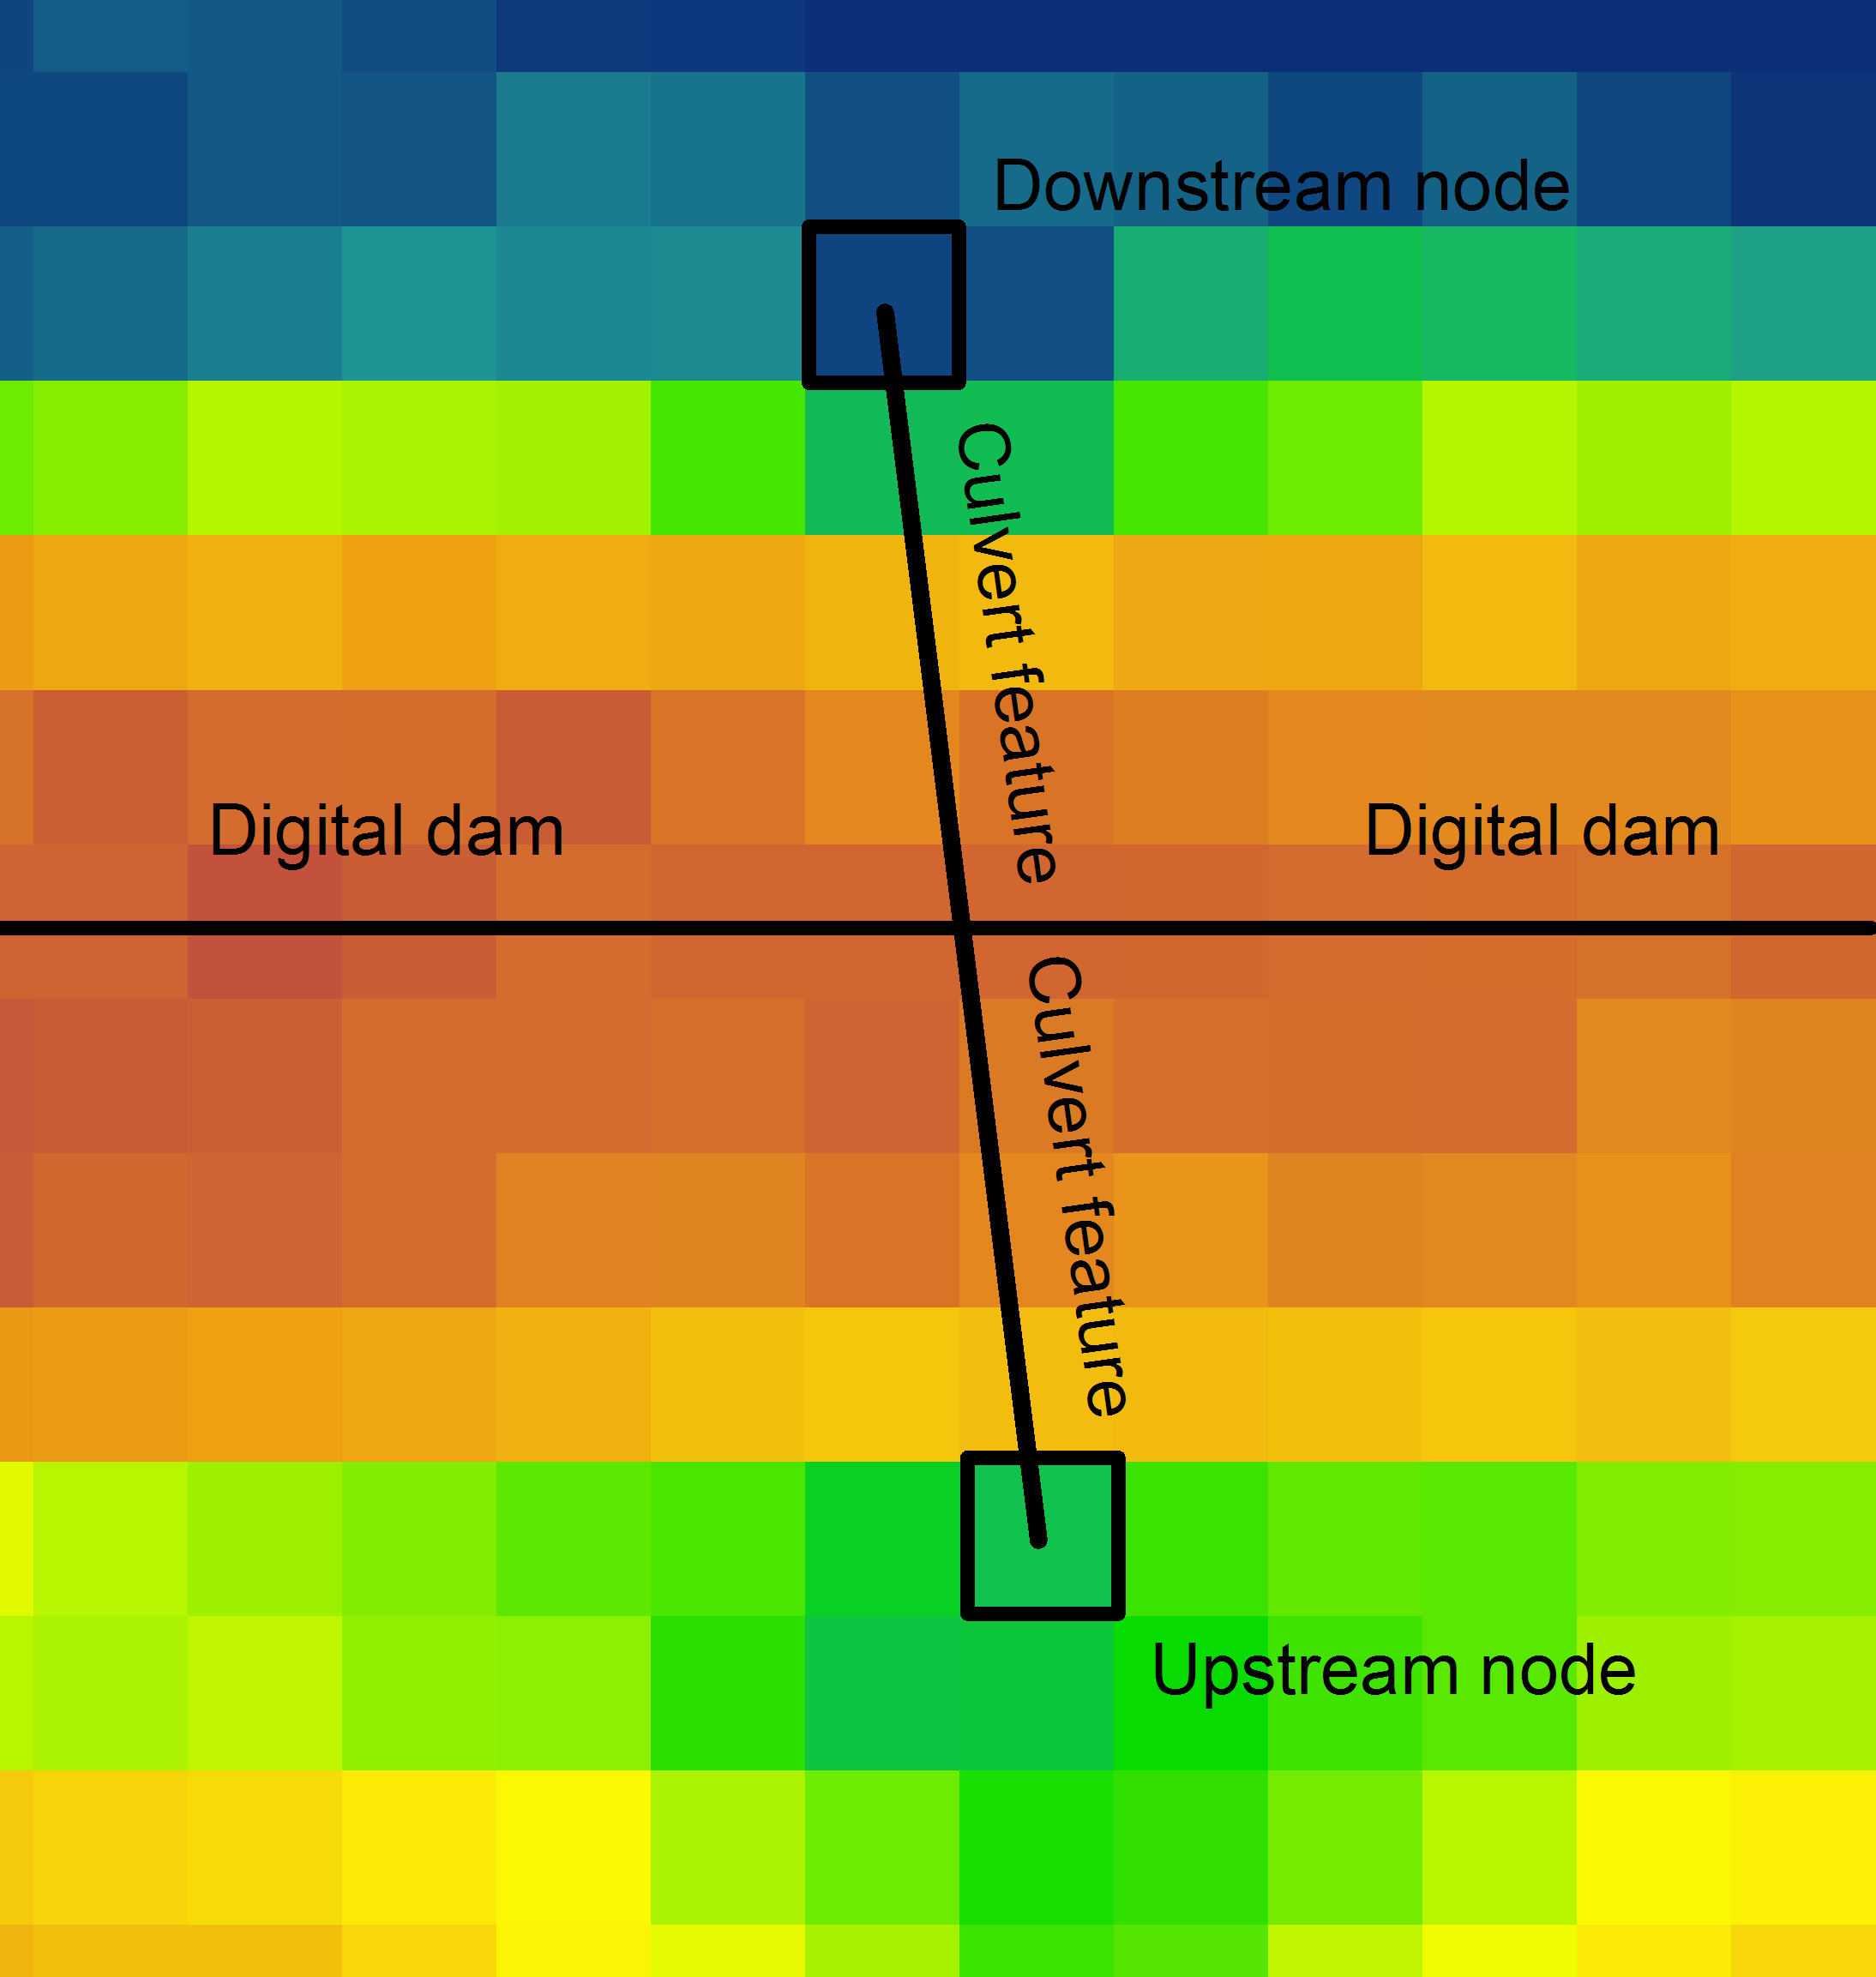
\includegraphics[width=0.5\textwidth,natwidth=2188,natheight=2306]{digitizingCulverts.png}
		\caption[Manual digitization of culvert features]{Manual digitization of culvert features. Gridded colors represent an elevation gradient---low elevations are represented by blue, mid-elevations by green and high elevations by red. The band of red running horizontally is the digital dam. The culvert feature must span the digital dam. The upstream and downstream nodes overlay low elevation pixels on either side of the digital dam.}
		\label{fig:digitizingCulverts}
	\end{figure}
\end{document}
